\documentclass[11pt]{article}

% Essential math packages
\usepackage{amsmath}
\usepackage{amssymb}
\usepackage{amsthm}
\usepackage{mathtools}

% Other useful packages
\usepackage{geometry}
\usepackage{graphicx}
\usepackage{enumitem}
\usepackage{float}
\usepackage{setspace}
\setstretch{1.2}     

% Page margins
\geometry{margin=1in}


% Title information
\title{[DRAFT] The Brachistrochrone Problem: a Finite Element Approach \thanks{Honors optional project for MATH 521}}

\author{Guizhong (Harry) Luo}
\date{03/2025}

\begin{document}
\maketitle 
\begin{abstract}
    The Brachistochrone problem seeks the path \(y(x)\) between two points that allows a particle sliding under gravity to travel in the minimum possible time. We present a numerical solution using the Finite Element Analysis (FEA) method. The continuous problem, formulated as minimizing the time functional 
    \begin{equation}
    T[y(x)] = \int_0^{x_f} \frac{\sqrt{1 + (y'(x))^2}}{\sqrt{2gy(x)}} dx,
    \label{eq:T}
    \end{equation}
        is discretized using P2 quadratic elements and approximated via Gaussian quadrature. This transforms the variational problem into a finite-dimensional nonlinear optimization problem, which is then optimized using the L-BFGS-B algorithm. 
    The numerical result nearly identical to the analytical cycloid solution, with a difference of \(0.1502\%\)
\end{abstract}


\section{Introduction}
!!TODO: Introduce the background of the problem, and derive the total time functional. State the analytical solution as a cycloid.

%%%%%%%%%%%%%%%%%%%%%%%%%%%%%%%%%%%%%%
\section{Finite Element Formulation}
    
    We employ quadratic (P2) finite elements to discretize the time functional and approximate the unknown path \(y(x)\).
    
    First, we divide the domain \( \left[0, x_f\right] \) into \(N \) uniform finite elements, each of length \( h = x_f / N \). We define a total of \(2N+1\) global nodes along the domain. The coordinate of the \(m\)-th global node (where \(m = 0, 1, \ldots, 2N\)) is given by
    \[ x_m = m \frac{h}{2}. \]
    Note that nodes with even indices \(m=2n\) ($n=0..N$) lie at the boundaries between elements (or domain ends), while nodes with odd indices \(m=2n+1\) ($n=0..N-1$) lie at the midpoints of the elements.
    
    An element \(e\) (where \(e = 1, 2, \ldots, N\)) is defined by three consecutive global nodes: a start node \(i = 2(e-1)\), a midpoint node \(j = 2e-1\), and an end node \(k = 2e\). The element thus spans the physical interval \( [x_i, x_k] \).
    
    We seek to determine the approximate vertical position \( y \) at each global node \(m\). Let \( y_m \approx y(x_m) \) denote the nodal value at node \(m\). These \( y_m \) values are the fundamental variables in our discretized problem. The boundary conditions fix the values at the first and last nodes:
    \[ y_{0} = y(x_{0}) = y(0) = 0 \quad , \quad y_{2N} = y(x_{2N}) = y(x_f) = y_f. \]
    The actual unknowns to be solved for are the values at the interior nodes ($m = 1, 2, \ldots, 2N-1$). We collect these unknown nodal values into the vector of degrees of freedom:
    \begin{equation}
    \mathbf{y_\text{int}} = \left[ y_1, y_2, \ldots, y_{2N-1} \right]^\top \in \mathbb{R}^{2N-1}.
    \label{eq:yint}
    \end{equation}

%%%%%%%%%%%%%%%%%%%%%%%%%%%%%%%    
\subsection{Local Coordinate System}
    
    To define approximations consistently within each element, it is convenient to map the physical coordinates \( x \) belonging to an element \(e\) (i.e., \(x \in [x_i, x_k]\)) to a dimensionless local coordinate \( \xi \in \left[-1,1\right] \). The mapping places the local origin \( \xi = 0 \) at the element's midpoint node \( x_j \):
    \begin{equation}
        x(\xi) \coloneqq \frac{x_{i} + x_k}{2} + \frac{x_k - x_{i}}{2} \xi =  x_j + \frac{h}{2} \xi. \label{eq:x(xi)}
    \end{equation}
    Here, the local coordinate \( \xi = -1 \) corresponds to the element's start node \( x_{i} \), \( \xi = 0 \) corresponds to the midpoint node \( x_j \), and \( \xi = 1 \) corresponds to the end node \( x_k \).
    
    The Jacobian of this transformation relates the physical and local differentials:
    \[ J = \frac{dx}{d\xi} = \frac{x_k - x_i}{2} = \frac{h}{2}. \]
    Hence, the differential transformation is
    \[
        dx = J d\xi = \frac{h}{2} d\xi.
    \]
    
%%%%%%%%%%%%%%%%%%%%%%%%%%%%%%%%%%%%%%%%%%%%%%    
\subsection{Quadratic Shape Functions for Approximating \( y(x) \) and \( y'(x) \) }
    
    Within element \(e\), let the nodal values corresponding to its start, mid, and end nodes be collected in the element nodal vector \( \mathbf{y}_{e} = \left[y_{i}, y_{j}, y_k\right]^{T}\), where \(i, j, k\) are the global indices for element \(e\). We approximate the function \( y(x) \) within this element using an interpolation \( y_h (x) \) based on these nodal values and quadratic shape functions of the local coordinate \( \xi \):
    \[
        y_h \left(\,x(\xi) \right) =  N_{1}(\xi) y_{i} + N_{2}(\xi) y_{j} + N_{3}(\xi) y_k.
    \]
    The quadratic shape functions \( N_1(\xi), N_2(\xi), N_3(\xi) \) must satisfy the interpolation property
    \[
        N_m(\xi_n) = \delta_{mn} \quad \text{for } m, n = 1, 2, 3,
    \]
    where we associate local node numbers $1, 2, 3$ with local coordinates
    \( \xi_1 = -1, \quad \xi_2 = 0, \quad \xi_3 = 1, \)
    and where \(\delta_{mn}\) denotes the Kronecker delta. This property ensures that the approximation \(y_h\) exactly matches the nodal values at the element's nodes: \( y_h(x_i) = y_i\), \( y_h(x_j) = y_j\), \( y_h(x_k) = y_k \).
    
    The unique quadratic polynomials satisfying these conditions are the Lagrange polynomials on \([-1, 1]\) for nodes at \(-1, 0, 1\):
    \[
    \begin{aligned}
        N_1(\xi) &= \frac{(\xi - 0)(\xi - 1)}{(-1 - 0)(-1 - 1)} = \frac{1}{2}\xi(\xi-1), \\
        N_2(\xi) &= \frac{(\xi - (-1))(\xi - 1)}{(0 - (-1))(0 - 1)} = \frac{(\xi+1)(\xi-1)}{-1} = 1 - \xi^2 ,\\
        N_3(\xi) &= \frac{(\xi - (-1))(\xi - 0)}{(1 - (-1))(1 - 0)} = \frac{1}{2}\xi(\xi+1).
    \end{aligned}
    \]
    The element approximation can be written compactly using vector notation:
    \begin{equation}
        y_h\left(x(\xi)\right) = \mathbf{N}(\xi) \cdot \mathbf{y}_e, \label{eq:yh}
    \end{equation}
    where \( \mathbf{N}(\xi) = [N_1(\xi), \; N_2(\xi), \; N_3(\xi)] \) is the vector of shape functions.
    
    Since the time functional \( T[y(x)] \) also depends on the derivative \( y'(x) \), we approximate this with the derivative of the interpolation, \( y'_h (x) \). Using the chain rule:
    \begin{equation*}
        y'_h (x) = \frac{dy_h}{dx}  = \frac{dy_h}{d\xi} \frac{d\xi}{dx}. 
    \end{equation*}
    Notice
    \[
        \frac{dy_h}{d\xi} = \frac{d}{d\xi} (\mathbf{N}(\xi) \cdot \mathbf{y}_e) = \left( \frac{d\mathbf{N}}{d\xi} \right) \cdot \mathbf{y}_e,
    \]
    where \( \frac{d\mathbf{N}}{d\xi} = \left[ \xi - \frac{1}{2},\; -2\xi,\; \xi + \frac{1}{2} \right] \).
    Using the inverse Jacobian \( \frac{d\xi}{dx} = 1/J = 2/h \), the approximation for the physical derivative becomes:
    \begin{equation}
        y'_h(x(\xi)) = \frac{2}{h} \left( \frac{d\mathbf{N}}{d\xi} \cdot \mathbf{y}_e \right)  = \frac{2}{h} \left( \left[ \xi - \frac{1}{2},\; -2\xi,\; \xi + \frac{1}{2} \right] \mathbf{y}_e \right). \label{eq:yhprime}
    \end{equation}

%%%%%%%%%%%%%%%%%%%%%%%%%%%%%%%%%%%%%%%%%%%%%
\subsection{Discretized Functional}
    
    For numerical optimization, we minimize the functional \( T^* \) which omits the constant factor \( \frac{1}{\sqrt{2g}} \) from the original total time functional (Eq.~\eqref{eq:T}) to get:
    \begin{equation}
        T^*[y(x)] = \int_0^{x_f} \sqrt{\frac{1 + (y'(x))^2}{y(x)}} dx .
    \label{eq:T*}
    \end{equation}
    We approximate this functional by replacing the exact function \( y(x) \) and its derivative \( y'(x) \) with their finite element approximations \( y_h (x) \) and \( y'_h (x) \). The integral over the full domain \( [0, x_f] \) is computed as the sum of integrals over each element \(e\):
    \begin{equation}
        T^*[y(x)] \approx T_h(\mathbf{y_\text{int}}) = \sum_{e=1}^{N} T_e^*(\mathbf{y}_e) \label{eq:Th}
    \end{equation}
    where \( T_e^* \) is the contribution from element \(e\), whose associated global nodes are \(i, j, k\):
    \begin{equation}
        T_e^*(\mathbf{y}_e) = \int_{x_{i}}^{x_{k}} \sqrt{\frac{1 + (y'_h(x))^2}{y_h(x)}} dx. \label{eq:Te*}
    \end{equation}
    The total approximate functional \( T_h \) is now expressed solely in terms of the nodal values \(\mathbf{y}_m\), specifically the unknown ones contained in the vector \(\mathbf{y_\text{int}}\) ( Eq.~\eqref{eq:yint}). 

%%%%%%%%%%%%%%%%%%%%%%%%%%%%%%%%%%%%%%%%%%%%%
\subsection{Element Integrals \( T^{*} _e \) }

We transform the integral \( T_e^* \) (Eq.~\eqref{eq:Te*}) to the local coordinate system using the change of variables \( x = x(\xi) \) and \( dx = J d\xi \), where \( \xi \in [-1, 1] \) . We also make the subsitution of the element approximations for \( y_h \) and \( y'_h \) as derived in Eq.~\eqref{eq:yh} and \eqref{eq:yhprime}.

Subsituting these into the integral for \( T^{*} _e \) (Eq.~\eqref{eq:Te*}): 
 
\[ 
    T_e^*(\mathbf{y}_e) = \int_{-1}^{1}\left(\frac{h}{2}\right) \sqrt{\frac{1 + \left[ \frac{2}{h} \left( \frac{d\mathbf{N}}{d\xi}(\xi) \cdot \mathbf{y}_e \right)  \right]^2}{\mathbf{N}(\xi) \cdot \mathbf{y}_e}}  d\xi
\]

For simplicity, we defined the following terms evaluated at a specific local coordinate \( \xi \) :  
\begin{align}
    &Y(\xi, \mathbf{y}_e) \coloneqq \mathbf{N}(\xi) \cdot \mathbf{y}_e \, , \\ 
    &Y'(\xi, \mathbf{y}_e) \coloneqq \frac{2}{h} \left( \frac{d\mathbf{N}}{d\xi}(\xi) \cdot \mathbf{y}_e \right) , \\ 
    &f_e(\xi, \mathbf{y}_e) \coloneqq \sqrt{\frac{1 + [Y'(\xi, \mathbf{y}_e)]^2}{Y(\xi, \mathbf{y}_e)}}. \label{eq:fe}
\end{align}

Then the element integral is written in compact form as  
\begin{equation}
    T_e^*(\mathbf{y}_e) = \int_{-1}^{1}  \frac{h}{2} f_e(\xi, \mathbf{y}_e) d\xi \label{eq:Te*compact}
\end{equation}

%%%%%%%%%%%%%%%%%%%%%%%%%%%%%%%%%%%%%%%%%%%%%
\section{Numerical integration via Gauss Quadrature}
The element integral in Eq.~\eqref{eq:Te*compact} is almost impossible to solve analytically, so we will approximate it using Gaussian Quadrature. The general form of Gaussian quadrature approximates an integral over \( \left[-1,1\right] \) as a weighted sum of the integrand evaluated at specific points within the interval:  
\[ 
    \int_{-1}^{1} g(\xi) d\xi \approx \sum_{p=1}^{P} w_p g(\xi_p) ,
\]
where \(P\) is the number of quadrature points, \(w_p\) are the quadrature weights, and \(\xi_p\) are the \( P \) distinct quadrature points within \( \left(-1,1\right) \) .

%%%%%%%%%%%%%%%%%%%%%%%%%%%%%%%%%%%%%%%%%%%%%
\subsection{Gauss-Legendre Quadrature for \( e > 1 \) }

For elements \( e = 2, 3, ..., N \), the path \(y_h(x) \)  is expected to be strictly positive with no end-point singularities. For such cases, standard Gauss-Legendre quadrature can be used. 

Let \( (\xi_{p}^{L}, w_{p}^{L}) \) ( for \( p = 1, \dots, P \) ) denote the Gauss-Legendre quadrature points and weights. The element integral \( T^{*_e}  \) for \( e > 1 \) is approximated as:  
\[ 
    T_e^*(\mathbf{y}_e) \approx \sum_{p=1}^{P} w_{p}^{L} \frac{h}{2} \left( f_e(\xi_{p}^{L}, \mathbf{y}_e)  \right).
\]
Subsituting the definition of \( f_e \) (Eq.~\eqref{eq:fe}), and including a small positive constant \( \epsilon \) to avoid division by zero, we have: 
\begin{equation}
    T_e^*(\mathbf{y}_e) \approx \sum_{p=1}^{P} w_{p}^{L} \frac{h}{2}  \left( \sqrt{\frac{1 + [Y'(\xi_{p}^{L}, \mathbf{y}_e)]^2}{ \max(Y(\xi_{p}^{L}, \mathbf{y}_e), \epsilon) }} \right) \quad \text{for } e = 2, \ldots, N \label{eq:Te*approx}
\end{equation}

%%%%%%%%%%%%%%%%%%%%%%%%%%%%%%%%%%%%%%%%%%%%%
\subsection{Gauss-Jacobi Quadrature for First Element}

Noticing the boundary condition \( y_{0} = 0, \) the first element \( e=1 \) introduces singularities. 

Recall the approximation within this element, where \( \mathbf{y}_1 = [y_0, y_1, y_2]^\top = [0, y_1, y_2]^\top \) :
\begin{align*}
    Y(\xi, \mathbf{y}_1) &= N_1(\xi)y_0 + N_2(\xi)y_1 + N_3(\xi)y_2 \\
    &= (1 - \xi^2)y_1 + \frac{1}{2}\xi(\xi+1)y_2 \\
    &= (1 + \xi)\left[(1-\xi) y_{1} + \frac{1}{2} \xi \, y_{2}\right].
\end{align*}
As \( \xi \to -1 \) , the term \( (1+\xi) \to 0 \). Denote \( H(\xi, \mathbf{y}_1) \coloneqq (1-\xi)y_1 + \frac{1}{2}\xi y_2 \). For a physical path, \( y_{1}, y_{2} > 0 \) and so \( H(-1, \mathbf{y}_1) = 2y_1 - 0.5y_2 \neq 0 \). 
Then the integrand as \( \xi \to -1 \) behaves like: 
\[ 
    f_1(\xi, \mathbf{y}_1) \propto \frac{1}{\sqrt{(1+\xi) H(\xi, \mathbf{y}_1)}} \propto (1+\xi)^{-1/2},
\]
reaching a singularity at \( \xi = -1 \). This invites the application of Gauss-Jacobi quadrature. 

Given an integrand in the form of \( f(x) = (1-x)^{\alpha} (1+x)^{\beta}  g(x), \, \alpha, \beta > -1  \), Gauss-Jacobi quadrature gives:  
\[ 
    \int_{-1}^{1} (1-x)^{\alpha} (1+x)^{\beta} g(x) dx \approx \sum_{i=1}^{P} w'_{i} g(x'_{i}).
\]
In our case,  \(\alpha=0, \beta=-1/2\), and so 
\[ 
    \int_{-1}^{1} (1+\xi)^{-1/2} g(\xi) d\xi \approx \sum_{p=1}^{P} w_{p}^{J} g(\xi_{p}^{J}) ,
\]
where \( \xi_{p}^{J} \) are the roots of the \( P\)-th degree Jacobi polynomial \( P_P^{(0, -1/2)}(\xi) \), and \( w_{p}^{J} \) are the corresponding weights for the weight function \( (1+\xi)^{-1/2} \).

To apply this rule, write 
\[ 
    T_1^*(\mathbf{y}_1) = \frac{h}{2} \int_{-1}^{1} \sqrt{\frac{1 + [Y'(\xi, \mathbf{y}_1)]^2}{Y(\xi, \mathbf{y}_1)}}  d\xi.
\]
Subsituting \( Y(\xi, \mathbf{y}_1) = (1+\xi) H(\xi, \mathbf{y}_1) \) : 
\begin{align*}
    T_1^*(\mathbf{y}_1) &= \int_{-1}^{1}  \frac{h}{2} \sqrt{\frac{1 + [Y'(\xi, \mathbf{y}_1)]^2}{(1+\xi) H(\xi, \mathbf{y}_1)}} d\xi \\
    &= \int_{-1}^{1} (1+\xi)^{-1/2}  \underbrace{\left[\frac{h}{2}  \sqrt{\frac{1 + [Y'(\xi, \mathbf{y}_1)]^2}{H(\xi, \mathbf{y}_1)}} \right]}_{g(\xi)} d\xi.
\end{align*}

Applying the Gauss-Jacobi quadrature rule, we have:
\[ 
    T_1^*(\mathbf{y}_1) \approx \sum_{p=1}^{P} w_{p}^{J} \left( \frac{h}{2}  \sqrt{\frac{1 + [Y'(\xi_{p}^{J}, \mathbf{y}_1)]^2}{H(\xi_{p}^{J}, \mathbf{y}_1)}} \right),
\] where \( H(\xi_{p}^{J}, \mathbf{y}_1) = (1-\xi_{p}^{J})y_1 + \frac{1}{2}\xi_{p}^{J} y_2 \) was previously defined. 

Introducing a small positive constant \( \epsilon \) to avoid division by zero, we replace the denominator with \( \max(H(\xi_{p}^{J}, \mathbf{y}_1), \epsilon) \), and thus  
\begin{equation}
    T_1^*(\mathbf{y}_1) \approx \sum_{p=1}^{P} w_{p}^{J}  \frac{h}{2} \left( \sqrt{\frac{1 + [Y'(\xi_{p}^{J}, \mathbf{y}_1)]^2}{ \max(H(\xi_{p}^{J}, \mathbf{y}_1), \epsilon) }} \right) \label{eq:T1*approx}
\end{equation}

Collecting the above, we arrive at the fininal discretized functional \( T_h \), which approximates the original functional \( T^{*}  \) using quadratic finite elements and Gaussian quadrature ( Eq.~\eqref{eq:Th}):
\begin{equation} 
    T^*[y(x)] \approx  T_h(\mathbf{y_\text{int}}) = T_1^*(\mathbf{y}_1) + \sum_{e=2}^{N} T_e^*(\mathbf{y}_e), \label{eq:T*approx}
\end{equation}
where  
\begin{align*}
    \mathbf{y}_1 &= [0, y_1, y_2]^\top, \\ 
    \mathbf{y}_e &= [y_{2(e-1)}, y_{2e-1}, y_{2e}]^\top \quad \text{for } e = 2, \ldots, N-1 \\ 
    \mathbf{y}_N &= [y_{2N-2}, y_{2N-1}, y_f]^\top.
\end{align*}
and the element contributions \( T^{*}_1 , T^*_e ( e >1)  \) were derived above ( Eq.~\eqref{eq:Te*approx}, \eqref{eq:T1*approx}). 


\section{Minimizing $ T_h $ for Fastest Descent}
The Brachistochrone problem is asking for a path of fastest descent, and so we seek to minimize the functional \( T^*[y(x)] \) ( Eq.~\eqref{eq:T*}) over all possible paths \( y(x) \). This will be approximated by minimizing the discretized functional \( T_h(\mathbf{y_\text{int}}) \) over all possible nodal values \( \mathbf{y_\text{int}} \). To be precise, we seek to solve the minimization problem:
\begin{align} 
     \min_{\mathbf{y_\text{int}} \in \mathbb{R}^{2N-1}} T_h(\mathbf{y_\text{int}}). \label{eq:minT}
\end{align}
We solve this by working with the gradient of the discretized functional 
 
\begin{align} 
    \nabla T_h(\mathbf{y_\text{int}}) = \left[ \frac{\partial T_h}{\partial y_1}, \frac{\partial T_h}{\partial y_2}, \ldots, \frac{\partial T_h}{\partial y_{2N-1}} \right]^\top. \label{eq:gradT} 
\end{align}

Since \( T_h = \sum_{e=1}^{N} T_e^* \), the gradient is obtained by summing contributions from elements that depend on \( y_m \):
\[ 
    \frac{\partial T_h}{\partial y_m} = \sum_{e \text{ s.t. node } m \text{ in element } e} \frac{\partial T_e^*}{\partial y_m}.
\]
It is computationally advantageous to first compute the gradient of each element's contribution \( T_e^* \) with respect to its own local nodal vector \( \mathbf{y}_e = [y_i, y_j, y_k]^T \). We denote this 3-component element gradient vector as:
\[ 
    \nabla_{\mathbf{y}_e} T_e^* = \left[ \frac{\partial T_e^*}{\partial y_i}, \frac{\partial T_e^*}{\partial y_j}, \frac{\partial T_e^*}{\partial y_k} \right]^T. 
\]
The global gradient \( \nabla T_h(\mathbf{y_\text{int}}) \) is then constructed by assembling these element gradient vectors.

\subsection{Gradient of $ T^{*}_e  $ for $ e > 1 $}
We start with the expression for \( T_e^* \) approximated using Gauss-Legendre quadrature (Eq.~\eqref{eq:Te*approx}):
\[ 
    T_e^*(\mathbf{y}_e) \approx \sum_{p=1}^{P} w_{p}^{L} \frac{h}{2} \left( \sqrt{\frac{1 + [Y'(\xi_{p}^{L}, \mathbf{y}_e)]^2}{ \max(Y(\xi_{p}^{L}, \mathbf{y}_e), \epsilon) }} \right) .
\]
Let \( F_p \coloneqq 1 + [Y'(\xi_p^L, \mathbf{y}_e)]^2 \) and \( Y_p \coloneqq \max(Y(\xi_p^L, \mathbf{y}_e), \epsilon) \). Then Eq.~\eqref{eq:Te*approx} becomes:  
\begin{align} 
    T_e^*(\mathbf{y}_e) \approx \sum_{p=1}^{P} w_{p}^{L} \frac{h}{2} \left( \sqrt{\frac{F_p}{Y_p}} \right) . \label{eq:Te*approx2}
\end{align}

To find $ \nabla_{\mathbf{y}_e} T_e^* $ , we need to compute \( \nabla_{\mathbf{y}_e} \left( \sqrt{F_p / Y_p} \right) \). Applying the chain rule and quotient rule, assuming \( Y_p > \epsilon \):
\begin{align*}
    \nabla_{\mathbf{y}_e} \left( \sqrt{\frac{F_p}{Y_p}} \right) &= \frac{1}{2 \sqrt{F_p / Y_p}} \nabla_{\mathbf{y}_e} \left( \frac{F_p}{Y_p} \right) \\
    &= \frac{1}{2 Y_p^2} \sqrt{\frac{Y_p}{F_p}} \left[ (\nabla_{\mathbf{y}_e} F_p) Y_p - F_p (\nabla_{\mathbf{y}_e} Y_p) \right].
\end{align*}
We then need the gradients of \( F_p \) and \( Y_p \) with respect to the element nodal vector \( \mathbf{y}_e \). Recall \( Y(\xi, \mathbf{y}_e) = \mathbf{N}(\xi) \cdot \mathbf{y}_e \) and \( Y'(\xi, \mathbf{y}_e) = \frac{2}{h} (\frac{d\mathbf{N}}{d\xi}(\xi) \cdot \mathbf{y}_e) \). 
\begin{itemize}
    \item Gradient of \( Y_p \): 
    \[ \nabla_{\mathbf{y}_e} Y_p = \nabla_{\mathbf{y}_e} (\mathbf{N}(\xi_p^L) \cdot \mathbf{y}_e) = \mathbf{N}(\xi_p^L)^T. \]
    Let \( \mathbf{N}_p \coloneqq \mathbf{N}(\xi_p^L)^T \).
    \item Gradient of \( F_p \): 
    \begin{align*}
        \nabla_{\mathbf{y}_e} F_p &= \nabla_{\mathbf{y}_e} (1 + [Y'(\xi_p^L, \mathbf{y}_e)]^2) = 2 Y'(\xi_p^L, \mathbf{y}_e) (\nabla_{\mathbf{y}_e} Y'(\xi_p^L, \mathbf{y}_e))
    \end{align*}
    where, gradient of \( Y' \) is:
    \[ \nabla_{\mathbf{y}_e} Y'(\xi_p^L, \mathbf{y}_e) = \nabla_{\mathbf{y}_e} \left( \frac{2}{h} \frac{d\mathbf{N}}{d\xi}(\xi_p^L) \cdot \mathbf{y}_e \right) = \frac{2}{h} \left(\frac{d\mathbf{N}}{d\xi}(\xi_p^L)\right)^T. \]
    Let \( \mathbf{N}'_p \coloneqq (\frac{d\mathbf{N}}{d\xi}(\xi_p^L))^T \). Then,
    \[ \nabla_{\mathbf{y}_e} F_p = 2 Y'(\xi_p^L, \mathbf{y}_e) \frac{2}{h} \mathbf{N}'_p. \]
\end{itemize}

Substituting these back, the gradient contribution from a single quadrature point is:
\[ 
    \nabla_{\mathbf{y}_e} \left( \sqrt{\frac{F_p}{Y_p}} \right) = \frac{1}{2 Y_p^2} \sqrt{\frac{Y_p}{F_p}} \left[ \left( 2 Y'_p \frac{2}{h} \mathbf{N}'_p \right) Y_p - F_p \mathbf{N}_p \right],
\]
where \( Y'_p = Y'(\xi_p^L, \mathbf{y}_e) \). The full element gradient vector \( \nabla_{\mathbf{y}_e} T_e^* \) for \( e >1 \) is obtained by summing these contributions over all quadrature points, weighted by \( w_p^L (h/2) \):
\begin{equation}
    \nabla_{\mathbf{y}_e} T_e^* \approx \sum_{p=1}^{P} w_{p}^{L} \left( \frac{h}{4 Y_p^2} \sqrt{\frac{Y_p}{F_p}} \left[ \left( 2 Y'_p \frac{2}{h} \mathbf{N}'_p \right) Y_p - F_p \mathbf{N}_p \right] \right). \label{eq:gradTe}
\end{equation}

\subsection{Gradient of \( T_1^* \) for the First Element (\( e = 1 \))}
For the first element, we used Gauss-Jacobi quadrature and the denominator \( H_p = \max(H(\xi_{p}^{J}, \mathbf{y}_1), \epsilon) \), where \( H(\xi, \mathbf{y}_1) = (1-\xi)y_1 + \frac{1}{2}\xi y_2 \) and \( \mathbf{y}_1 = [0, y_1, y_2]^T \).
\[ 
    T_1^*(\mathbf{y}_1) \approx \sum_{p=1}^{P} w_{p}^{J} \frac{h}{2} \left( \sqrt{\frac{F_p}{H_p}} \right) ,
\]
where \( F_p = 1 + [Y'(\xi_p^J, \mathbf{y}_1)]^2 \). This gradient calculation follows the same structure, requiring \( \nabla_{\mathbf{y}_1} F_p \) and \( \nabla_{\mathbf{y}_1} H_p \). Note that the gradient is with respect to \( \mathbf{y}_1 = [y_0, y_1, y_2]^T \).

\begin{itemize}
    \item Gradient of \( H_p \): Since \( H \) does not depend on \( y_0 \), and assuming $ H(\xi^{J}_p , y_{1}) > \epsilon $, we have:
    \[ \nabla_{\mathbf{y}_1} H_p = \left[ \frac{\partial H_p}{\partial y_0}, \frac{\partial H_p}{\partial y_1}, \frac{\partial H_p}{\partial y_2} \right]^T = \left[ 0, \quad 1-\xi_p^{J}, \quad \frac{1}{2}\xi_p^{J} \right]^T. \]
    Let \( \mathbf{H}'_p \coloneqq \nabla_{\mathbf{y}_1} H_p \).
    \item Gradient of \( F_p \): We need \( \nabla_{\mathbf{y}_1} Y'(\xi_p^J, \mathbf{y}_1) \). Recall 
    \( Y'(\xi, \mathbf{y}_1) = \frac{2}{h} ( -2\xi y_1 + (\xi + 1/2) y_2 ) \).
    \[ \nabla_{\mathbf{y}_1} Y'(\xi_p^J, \mathbf{y}_1) = \left[ \frac{\partial Y'}{\partial y_0}, \frac{\partial Y'}{\partial y_1}, \frac{\partial Y'}{\partial y_2} \right]^T = \frac{2}{h} \left[ 0, \quad -2\xi_p^{J}, \quad \xi_p^{J}+\frac{1}{2} \right]^T. \]
    Let \( \mathbf{Y}''_{p,1} \coloneqq \nabla_{\mathbf{y}_1} Y'(\xi_p^J, \mathbf{y}_1) \). Then,
    \[ \nabla_{\mathbf{y}_1} F_p = 2 Y'(\xi_p^J, \mathbf{y}_1) (\nabla_{\mathbf{y}_1} Y'(\xi_p^J, \mathbf{y}_1)) = 2 Y'_p \mathbf{Y}''_{p,1}. \]
\end{itemize}

The gradient contribution from a single Gauss-Jacobi point is:
\[ 
    \nabla_{\mathbf{y}_1} \left( \sqrt{\frac{F_p}{H_p}} \right) = \frac{1}{2 H_p^2} \sqrt{\frac{H_p}{F_p}} \left[ (\nabla_{\mathbf{y}_1} F_p) H_p - F_p (\nabla_{\mathbf{y}_1} H_p) \right],
\]
where \( Y'_p = Y'(\xi_p^J, \mathbf{y}_1) \). Summing over the quadrature points gives the element gradient vector \( \nabla_{\mathbf{y}_1} T_1^* \):
\begin{equation}
    \nabla_{\mathbf{y}_1} T_1^* \approx \sum_{p=1}^{P} w_{p}^{J} \left( \frac{h}{4 H_p^2} \sqrt{\frac{H_p}{F_p}} \left[ (2 Y'_p \mathbf{Y}''_{p,1}) H_p - F_p \mathbf{H}'_p \right] \right). \label{eq:gradT1}
\end{equation}


\subsection{Global Gradient Assembly}

The global gradient vector \( \nabla T_h(\mathbf{y_\text{int}}) \in \mathbb{R}^{2N-1} \) is assembled by summing the contributions from the relevant element gradient vectors. Let \( \mathbf{G} \coloneqq \nabla T_h(\mathbf{y_\text{int}}) \) denote this global vector, indexed such that its $m$-th component is \( G_m = \partial T_h / \partial y_m \) for \( m=1, \dots, 2N-1 \). Since \( T_h = \sum_{e=1}^{N} T_e^* \), differentiating with respect to \( y_m \) yields:
\[
    G_m = \frac{\partial T_h}{\partial y_{m}} = \frac{\partial}{\partial y_{m}} \left( \sum_{e=1}^{N} T_e^*(\mathbf{y}_e) \right) = \sum_{e \text{ s.t. node } m \text{ in element } e} \frac{\partial T_e^*}{\partial y_{m}}.
\]
The assembly process calculates \( \mathbf{G} \) by iterating through the elements: Initialize \( \mathbf{G} \) as a zero vector. Then, for each element \( e = 1, \dots, N \):
\begin{enumerate}
    \item Compute the 3-component element gradient vector \( \mathbf{g}_e \coloneqq \nabla_{\mathbf{y}_e} T_e^* = [g_{e,i}, g_{e,j}, g_{e,k}]^T \) using Eq. \eqref{eq:gradTe} (for \(e > 1\)) or Eq. \eqref{eq:gradT1} (for \(e=1\)), where \(i=2(e-1), j=2e-1, k=2e\) are the global node indices for the element.
    \item Add the components of \( \mathbf{g}_e \) to the global gradient vector \( \mathbf{G} \) at entries corresponding to the \textbf{unknown} interior nodes:
    \begin{itemize}
        \item If node \( i \) is an interior node (i.e., \( i > 0 \)), perform the update: \( G_i \leftarrow G_i + g_{e,i} \).
        \item Node \( j \) is always an interior node (\( j = 2e-1 \)), perform the update: \( G_j \leftarrow G_j + g_{e,j} \).
        \item If node \( k \) is an interior node (i.e., \( k < 2N \)), perform the update: \( G_k \leftarrow G_k + g_{e,k} \).
    \end{itemize}
\end{enumerate}
After iterating through all elements, the vector \( \mathbf{G} \) holds the complete gradient \( \nabla T_h(\mathbf{y_\text{int}}) \).
\section{Numerical Solution and Results}

With the discretized objective function \( T_h(\mathbf{y_\text{int}}) \) (Eq.~\eqref{eq:Te*approx}) and its gradient \( \nabla T_h(\mathbf{y_\text{int}}) \) (Eq.~\eqref{eq:gradT}) derived, the Brachistochrone problem is reduced to a finite-dimensional optimization problem (Eq.~\eqref{eq:minT}). We solve this numerically using the Limited-memory Broyden-Fletcher-Goldfarb-Shanno (L-BFGS-B) algorithm, which iteratively minimizes \( T_h(\mathbf{y_\text{int}}) \) using function and gradient evaluations.

For an initial guess, we adopt a circular arc path, as considered by Galileo.  The physical constraint \(y(x) \ge 0\) is enforced by setting lower bounds \( y_m \ge \epsilon \) for all unknown nodal values within the L-BFGS-B solver.

We implemented this P2 FEA approach with $ N = 20 $ quadratic elements, $ P = 10 $ Gauss quadrature points per element, and $ \epsilon = 1e-15 $.  The optimization yields the optimal nodal values $ \mathbf{y_\text{int}}^{*} $, and the resulting path, reconstructed via quadratic interpolation, represents our FEA solution, visualized in Figure \ref{fig:1}.

Figure \ref{fig:1} demonstrates excellent agreement between the P2 FEA solution and the analytical cycloid. The FEA-approximated minimum descent time, \texttt{FEA T = 0.806744}, closely matches the theoretical minimum, \texttt{Exact T = 0.805564}, with a difference of only \(0.1502\%\).
\begin{figure}
    \centering
    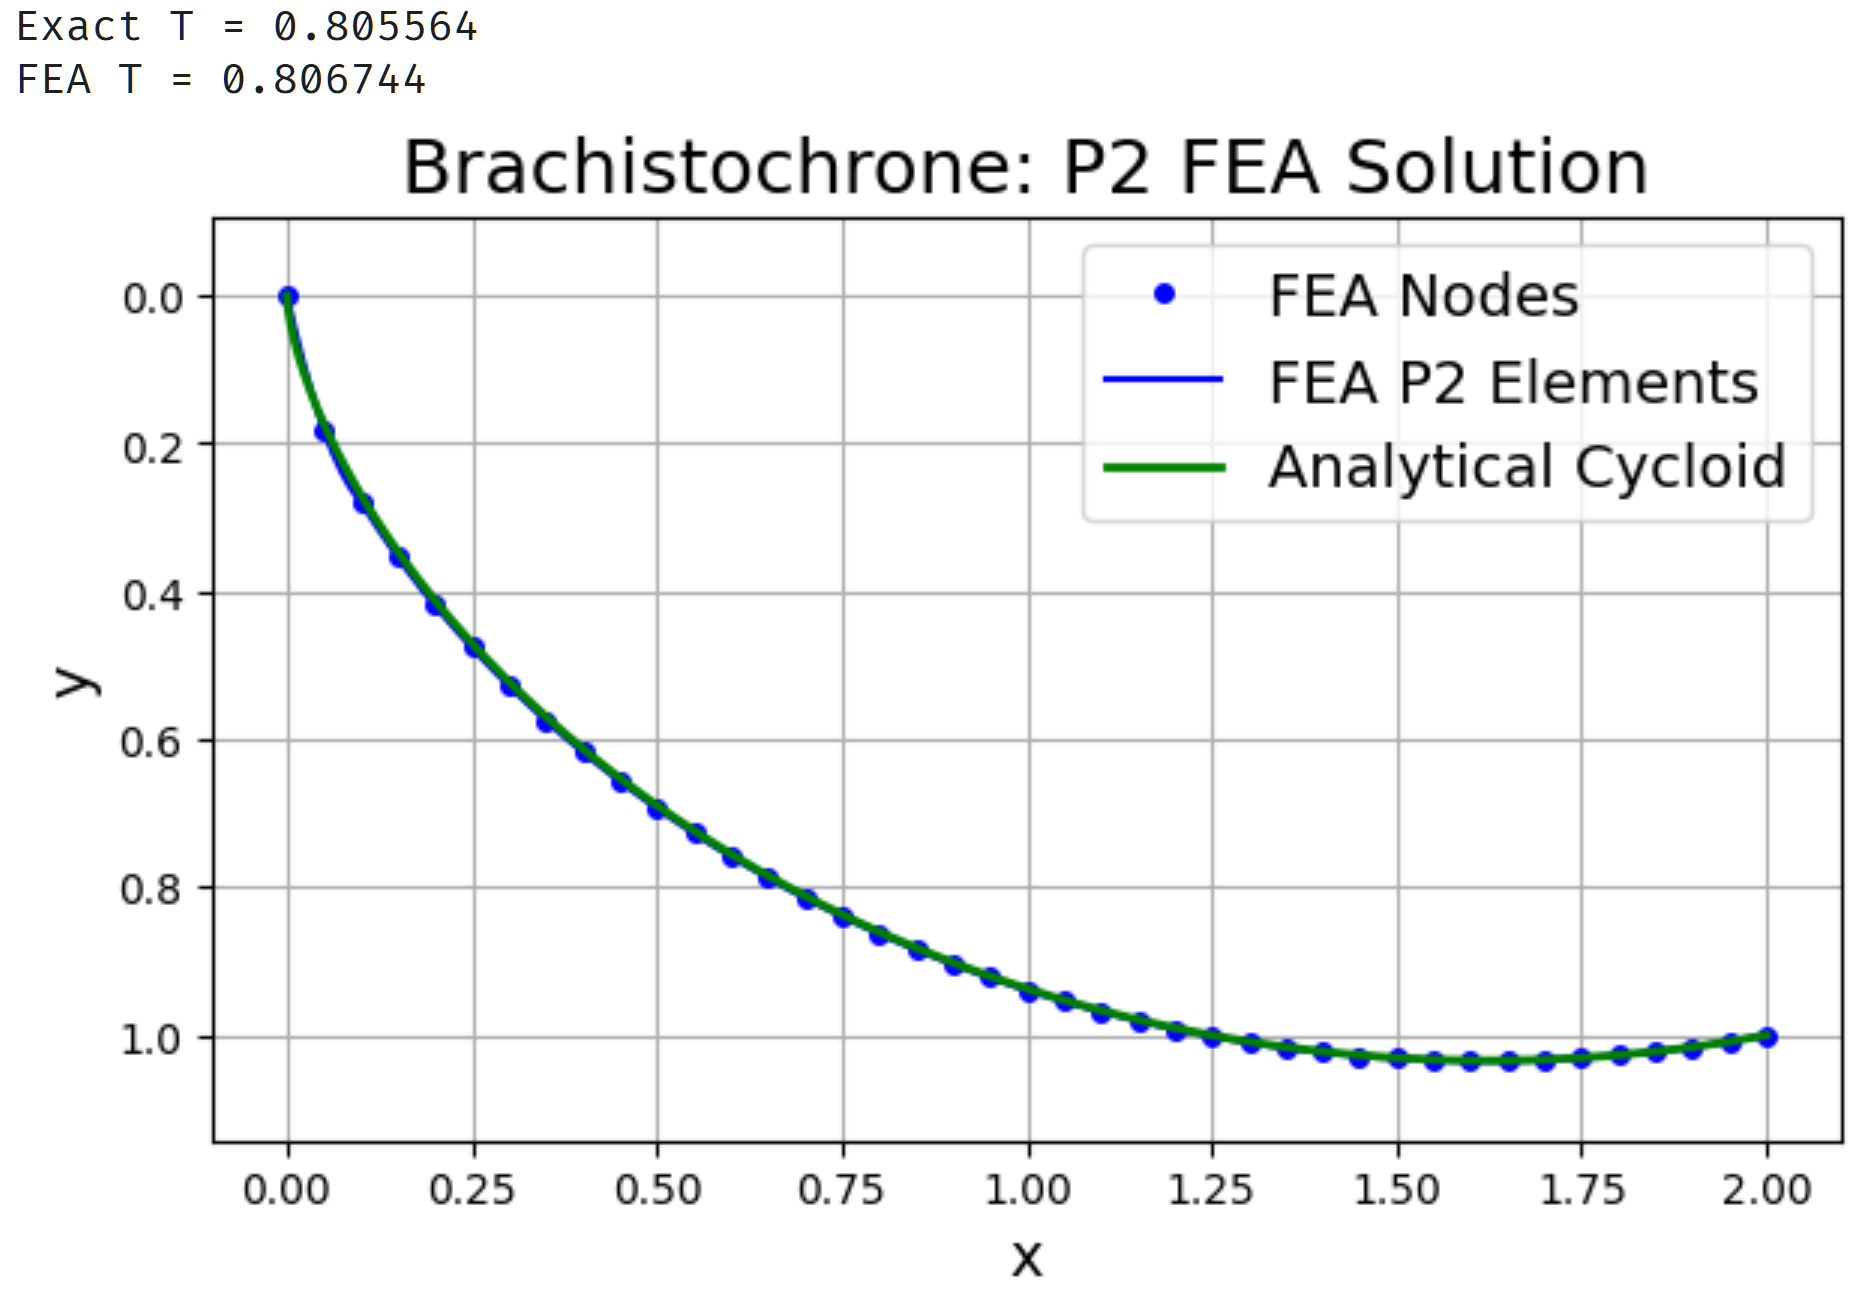
\includegraphics[width=0.6\linewidth]{FEA_plot.png}
    \caption{Comparison of the P2 FEA solution with the analytical cycloid solution}
    \label{fig:1}
\end{figure}

\newpage
\section*{Appendix}
Code used for Numrical Solution:

\begin{verbatim}
    import numpy as np
import matplotlib.pyplot as plt
from scipy.optimize import minimize, brentq
from scipy.special import roots_jacobi

# --- Configuration ---
QUAD = 10  # Quadrature points
EPS = 1e-15 #epsilon
xi_leg, w_leg = np.polynomial.legendre.leggauss(QUAD)
xi_jac, w_jac = roots_jacobi(QUAD, 0, -0.5)  # For singularity at x=0

def shape(xi):
    """P2 shape functions and derivatives"""
    N = np.array([0.5*xi*(xi-1), 1-xi**2, 0.5*xi*(xi+1)])
    dN = np.array([xi-0.5, -2*xi, xi+0.5])
    return N, dN

def element(y, h, first=False):
    """Element T* and gradient calculation"""
    T, g = 0, np.zeros(3)
    xi, w = (xi_jac, w_jac) if first else (xi_leg, w_leg)

    for i in range(len(xi)):
        N, dN = shape(xi[i])
        Y = max(y @ N, EPS)
        Yp = y @ dN * (2/h)
        F = 1 + Yp**2
        dF = 2 * Yp * (2/h) * dN

        if first:
            # First element (singularity)
            G = max(y[1]*(1-xi[i]) + y[2]*0.5*xi[i], EPS)
            T += w[i] * np.sqrt((F+EPS)/G) * (h/2)
            dG = np.array([0, 1-xi[i], 0.5*xi[i]])
            fac = (h/4) * np.sqrt(G/(F+EPS)+EPS) / (G**2+EPS)
            g += w[i] * fac * ((dF*G) - (F*dG))
        else:
            # Regular element
            T += w[i] * np.sqrt((F+EPS)/Y) * (h/2)
            fac = (h/4) * np.sqrt(Y/(F+EPS)+EPS) / (Y**2+EPS)
            g += w[i] * fac * ((dF*Y) - (F*N))

    return T, g

def global_calc(y_unk, h, yf, N):
    """Global T* and gradient assembly"""
    y = np.zeros(2*N+1)
    y[1:-1], y[-1] = y_unk, yf

    T, g = 0, np.zeros(len(y_unk))

    for i in range(1, N+1):
        idx = [2*(i-1), 2*i-1, 2*i]
        Ti, gi = element(y[idx], h, first=(i==1))
        T += Ti

        if idx[0] > 0: g[idx[0]-1] += gi[0]
        g[idx[1]-1] += gi[1]
        if idx[2] < 2*N: g[idx[2]-1] += gi[2]

    return T, g

class BrachSolver:
    def __init__(self, xf, yf, N):
        self.xf, self.yf, self.N, self.h = xf, yf, N, xf/N

    def obj(self, y): return global_calc(y, self.h, self.yf, self.N)[0]
    def grad(self, y): return global_calc(y, self.h, self.yf, self.N)[1]

    def solve(self):
        # Initial circular arc guess
        x = np.linspace(0, self.xf, 2*self.N+1)
        hc = (self.xf**2 + self.yf**2)/(2*self.xf)
        y0 = np.sqrt(np.maximum(hc**2 - (x[1:-1]-hc)**2, 0))

        # Run optimizer
        res = minimize(
            self.obj, y0, jac=self.grad, method='L-BFGS-B',
            bounds=[(EPS, None)]*len(y0),
            options={'disp': True, 'gtol': 1e-7}
        )

        if res.success:
            y_sol = np.zeros(2*self.N+1)
            y_sol[1:-1], y_sol[-1] = res.x, self.yf
            return {'y': y_sol, 'T': res.fun/np.sqrt(2*9.81), 'success': True}
        return {'success': False}

def draw_quadratic_elements(x_nodes, y_nodes, num_points=10):
    """Draw smooth quadratic elements"""
    x_smooth = []
    y_smooth = []

    for i in range(0, len(x_nodes)-2, 2):
        # Extract the 3 nodes of this element
        x_elem = x_nodes[i:i+3]
        y_elem = y_nodes[i:i+3]

        # Map to reference element [-1, 1]
        h_elem = x_elem[2] - x_elem[0]
        x_mid = (x_elem[0] + x_elem[2])/2

        # Generate points within the element
        xi_local = np.linspace(-1, 1, num_points)
        x_local = []
        y_local = []

        for xi in xi_local:
            # Shape functions at xi
            N1 = 0.5*xi*(xi-1)
            N2 = 1-xi**2
            N3 = 0.5*xi*(xi+1)

            # Compute physical coordinates using shape functions
            x = x_elem[0]*N1 + x_elem[1]*N2 + x_elem[2]*N3
            y = y_elem[0]*N1 + y_elem[1]*N2 + y_elem[2]*N3

            x_local.append(x)
            y_local.append(y)

        x_smooth.extend(x_local)
        y_smooth.extend(y_local)

    return np.array(x_smooth), np.array(y_smooth)

def cycloid(xf, yf):
    """Find analytical cycloid parameters"""
    f = lambda t: (t-np.sin(t))/(1-np.cos(t)+EPS) - xf/yf
    theta = brentq(f, 1e-9, 2*np.pi-1e-9)
    a = yf/(1-np.cos(theta))
    return a, theta

# Main execution
if __name__ == "__main__":
    xf, yf = 2.0, 1.0 
    N = 20
    g = 9.81

    # Analytical solution
    a, theta = cycloid(xf, yf) 
    T_exact = theta * np.sqrt(a/g) 
    print(f"Exact T = {T_exact:.6f}") 
    # FEA solution
    solver = BrachSolver(xf, yf, N)
    result = solver.solve()

    if result['success']:
        print(f"FEA T = {result['T']:.6f}")

        # Plot
        plt.figure(figsize=(7, 4))
        x = np.linspace(0, xf, 2*N+1)

        # Plot nodes
        plt.plot(x, result['y'], 'bo', ms=4, label='FEA Nodes')

        # Plot quadratic elements
        x_smooth, y_smooth = draw_quadratic_elements(x, result['y'], num_points=20)
        plt.plot(x_smooth, y_smooth, 'b-', lw=1.5, label='FEA P2 Elements')

        # Plot analytical solution
        t = np.linspace(0, theta, 200)
        plt.plot(a*(t-np.sin(t)), a*(1-np.cos(t)), 'g-', lw=2, label='Analytical Cycloid')

        plt.xlabel('x', fontsize=14) 
        plt.ylabel('y', fontsize=14) 
        plt.title('Brachistochrone: P2 FEA Solution', fontsize=18)
        plt.gca().invert_yaxis()
        plt.grid(True)
        plt.axis('equal')
        plt.legend(fontsize=14)  
        plt.show()

\end{verbatim}





\end{document}
